%%% Preamble
% Article class of KOMA-script with 11pt font and a4 format
\documentclass[paper=a4, fontsize=11pt]{scrartcl}	
\usepackage[T1]{fontenc}
\usepackage{fourier}

% English language/hyphenation
\usepackage[english]{babel}

% Better typography
\usepackage[protrusion=true,expansion=true]{microtype}

% Math packages
\usepackage{amsmath,amsfonts,amsthm}

% Enable pdflatex
\usepackage[pdftex]{graphicx}
\usepackage{url}

\usepackage{caption}
\usepackage{subcaption}

% Tables
\usepackage{multirow}

%%% Custom sectioning (sectsty package)
% Custom sectioning (see below)
\usepackage{sectsty}
% Change font of al section commands
\allsectionsfont{\centering \normalfont\scshape}

\setlength{\parindent}{25pt}

%%% Custom headers/footers (fancyhdr package)
\usepackage{fancyhdr}
\pagestyle{fancyplain}

% No page header
\fancyhead{}

% You may remove/edit this line 
\fancyfoot[L]{\small SIGB Final Hand-in}
\fancyfoot[C]{} % Empty
\fancyfoot[R]{\thepage} % Pagenumbering
\renewcommand{\headrulewidth}{0pt} % Remove header underlines
\renewcommand{\footrulewidth}{0pt} % Remove footer underlines
\setlength{\headheight}{13.6pt}


%%% Equation and float numbering
\numberwithin{equation}{section} % Equationnumbering: section.eq#
\numberwithin{figure}{section} % Figurenumbering: section.fig#
\numberwithin{table}{section} % Tablenumbering: section.tab#


%%% Maketitle metadata
\newcommand{\horrule}[1]{\rule{\linewidth}{#1}} % Horizontal rule

\title{
	%\vspace{-1in} 	
	\usefont{OT1}{bch}{b}{n}
	\normalfont \normalsize \textsc{IT University of Copenhagen} \\ [25pt]
	\horrule{0.5pt} \\[0.4cm]
	\huge Introduction to Graphics and Image Analysis Final Report \\
	\horrule{2pt} \\[0.5cm]
}

\author{
	\normalfont 
	\normalsize
	Miroslav Zoricak (mzor@itu.dk) \\[-3pt]
	\normalsize
	Arin Agha Seyed Hashem Kadkhoda (aseh@itu.dk) \\[-3pt]
	\normalsize
	\today
}

\date{}


%%% Begin document
\begin{document}
\maketitle
\newpage
\tableofcontents
\newpage
\section{Introduction}

In this assignment we were tasked to explore various applications of homographies. Like the first assignment, to obtain our goal we used Python and OpenCV as a toolkit. The purpose is to learn how to use homographies because it’s related to both computer vision and computer graphics applications and is in general very useful for many applications. 

In this assignment we covered some used of homographies like point transfers, texture mapping, camera calibration and some of the benefits of having a calibrated camera, however we can’t cover all of the homographies uses because the time available for us is limited and there is extreme range of situation that homographies can be useful.



\pagebreak
\section{Eye Tracker}

\subsection{Introduction}
We were tasked with the construction of a software eye tracker. In the following text we describe our approach to this challenge, the methods we have used, and the results we have obtained.  We have built the eye tracker using Python and OpenCV as a toolkit. The purpose of the eye tracker is to correctly and accurately detect the eye (pupil, iris) and glints on the eye in every image where there is an eye and detect nothing if there is no eye present in the image.

In general, eye tracker algorithms are reducing a huge amount of data (typical 640x480 RGB image is almost 1MB of uncompressed data) to just a few values representing the location and radius of pupil, iris and various glints. Therefore there must be many ways of performing this reduction, some better than others. Our goal in this report is to describe the approach we have taken to solving this problem, which algorithms we have used and what observations and results we have achieved.

As with any work, compromises have to be made and the time available for us to solve this problem is limited. Therefore at some point we must stop looking for more advanced improvements, even though this process could theoretically go on forever. In this report we present the results we have achieved and interesting observations we have made during the process and evaluate how our proposed solution performed.

We wanted to make the tracker as robust as possible, without the need for per-sequence parameterization. It should perform reasonably well without needing any parameter tweaking. Therefore most our efforts have been targeted at eliminating the parameterization in as many places as possible.

The hardest matter that we have faced has been to build the tracker as solid as possible, without the need for per-sequence parameterization. It should work in all circumstances as good as possible. This is of course especially hard.

\subsection{Method}

We started identifying common patterns occurring in the sample sequences that we would use to test our eye tracker on. Based on these patterns we have then formed our ideas of how should the software perform the detection. The patterns we have observed are as follows:

\begin{enumerate}

\item All sequences are taken with an IR camera, therefore the image has low chromaticity, but high luminance response. Therefore color could not be used to detect the eye, only the intensity.
\item Similarly, all sequences have resolution of 640x480 pixels, as a result of being taken with a web cam.
\item In all sequences there is one and only one eye, even though blinks can occur, so no pupil is visible.
\item All sequences are shorter than 30 seconds.

\end{enumerate}

We have built our eye tracker with these assumptions, so if any of them is broken (apart from 4.), our software will probably struggle to give a correct result. Another consideration we have made is that the performance is not the objective at this stage, so we have preferred solutions that are correct and complete over solutions that just are fast. That being said, the software could still be optimized for performance and lower memory footprint removing a lot of repetition of the same calculations and code that has been introduced to enable parametrization of our partial functions.

During our work we were looking for solutions that would require as few parameters as possible, ideally none. This has led us to use k-means to obtain parameters for thresholding, which are quite volatile and trade them for parameters to k-means, which are far less volatile. In fact we have been able to use the single value for all sequences.

Similarly we have looked at all improvements to the algorithm by comparing the results of our test (Described in Section 3 Results) to the best previously achieved result. If the proposed improvement was better in all cases (increased the number of correct detections) then it was accepted, if this was not the case, it was rejected.

The following subsections detail the concrete methods we have applied to get pupil, iris and glints from the images. All of them work on gray scale images.

\subsubsection{Pupil Detection}
For pupil detection we start off by computing k-means for a downsized gray scale image. Kmeans algorithm iteratively partitions all the pixels into k clusters, where each pixel belongs to a cluster with the nearest mean. In praxis this means that it will separate different levels of gray into separate regions. You can see an example of k-means clustering on  \ref{fig:kmeans}.

\begin{figure}[h!]
\centering
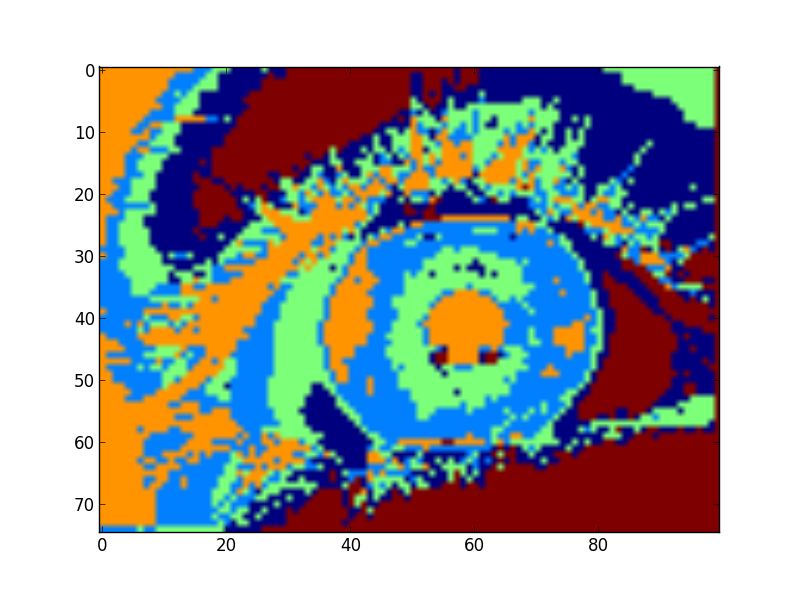
\includegraphics[width=\columnwidth]{final/images/k-means.png}
\caption{k-means clustering}
\label{fig:kmeans}
\end{figure}

Since the pupil is usually very dark, it is (in most cases) safe to assume that it will be contained in the first cluster (the darkest). Therefore k-means can be used in this way to circumvent the need of setting threshold values for the thresholding function that comes next. Instead of a pre-chosen threshold we simply use the value of the first cluster. That ensures that the threshold will be set to contain the darkest values in the image (and by extension likely the pupil). The thresholded image obtained using the k-means from Figure \ref{fig:kmeans} can be seen in Figure \ref{subfig:thresh}. 

\begin{figure}[h!]
	\centering
	
	\begin{subfigure}[b]{0.5\textwidth}
		\centering
		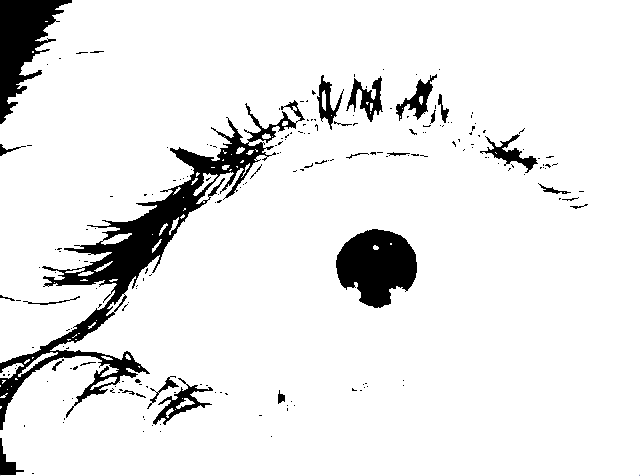
\includegraphics[width=\textwidth]{final/images/thresh.png}
		\caption{After Thresholding}
		\label{subfig:thresh}
	\end{subfigure}%
	~
	\begin{subfigure}[b]{0.5\textwidth}
		\centering
		
\includegraphics[width=\textwidth]{final/images/open.png}
		\caption{After Opening}
		\label{subfig:open}
	\end{subfigure}
	
	\caption{Thresholding and Opening}
	\label{fig:threshopen}
\end{figure}

After thresholding we perform opening.  Opening is a morphological operation that consists of performing erosion followed by dilation. This cleans up the image, removing noise and speckles. You can see this in the Figure \ref{subfig:open}.

This gives us an image that is well suited for blob analysis. We perform this in two steps. First we remove all blobs which are bigger than 30\% of the image area or smaller than 0.2\% of the entire image. This removes blobs that are most likely not pupil. Second fit an ellipse to the contour and then we compare the ratio between the two radii of that ellipse. That removes all matches that are too elliptical. The pupil is usually more like a circle, but can be slightly elliptical when the user is looking to the side.

The last step we perform is ordering, we order all detected ellipses by increasing extend. This ensures that the most contained blobs come first. In most cases this should prioritize well contained blobs (such as the pupil) over false positives, and all the other detection functions just take the first result from pupil detection.

We have also implemented a failsafe mechanism, that, in absence of any pupils detected, can iteratively call the getPupils() function with lower values of k, which results in better performance in sequences with high contrast. In particular in sequence 8 this change alone has improved the detection rate from 0\% to 62.5\% in the testing frames.

\subsubsection{Iris Detection}

For iris detection we start with the position of the pupil detected previously. First we filter the image using the Sobel filter. Then we use the filtered image to calculate orientation (Figure \ref{subfig:quiver}) and magnitude (Figure \ref{subfig:magnitude}) of the gradient image. 

\begin{figure}[h!]
	\centering
	
	\begin{subfigure}[b]{0.5\textwidth}
		\centering
		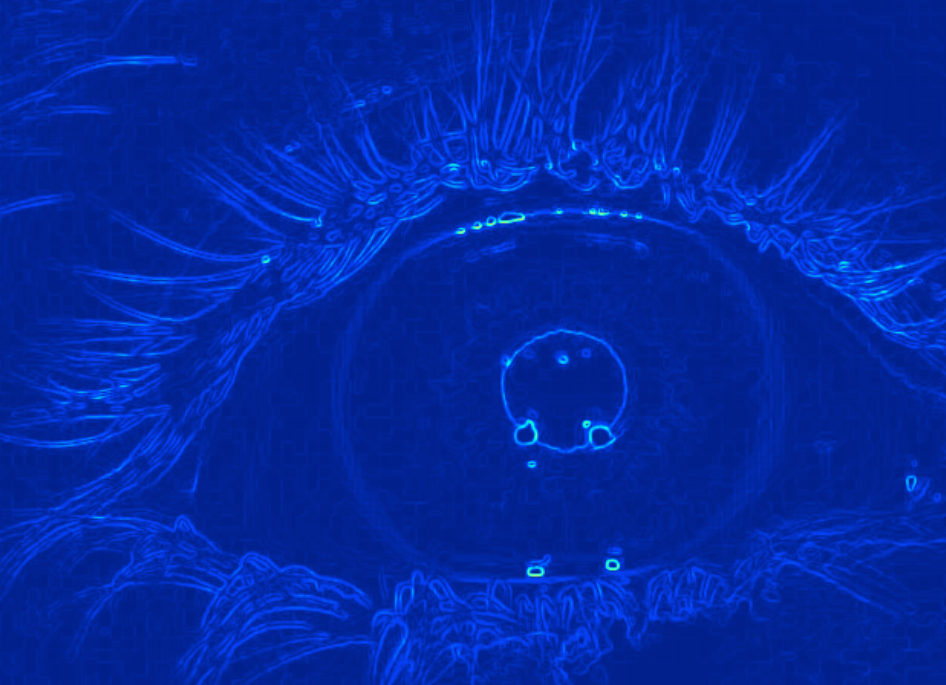
\includegraphics[width=\textwidth]{final/images/magnitude.png}
		\caption{Magnitude}
		\label{subfig:magnitude}
	\end{subfigure}%
	~
	\begin{subfigure}[b]{0.5\textwidth}
		\centering
		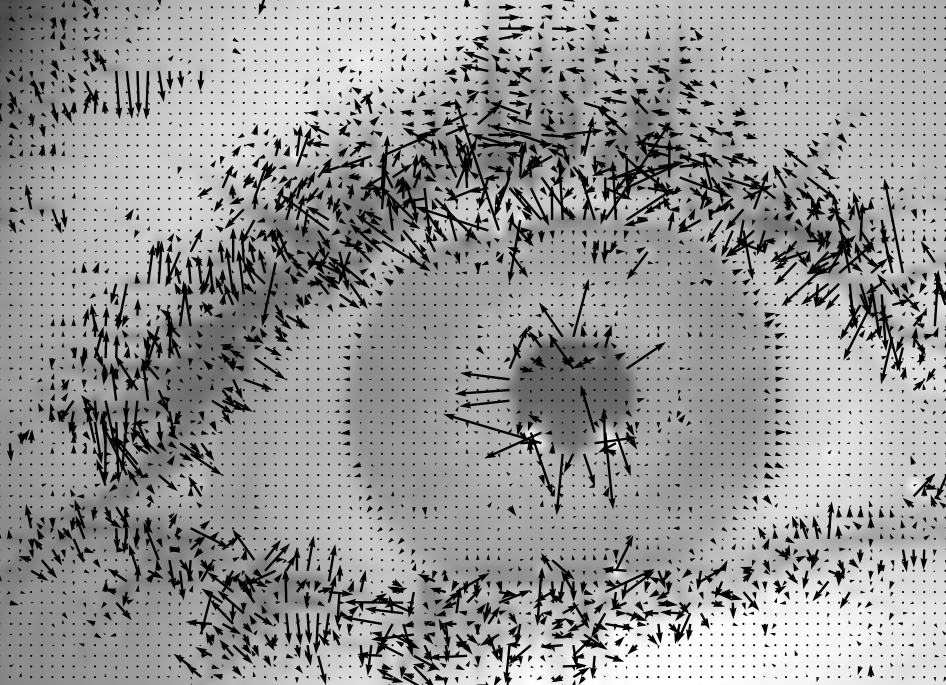
\includegraphics[width=\textwidth]{final/images/quiver.png}
		\caption{Orientation}
		\label{subfig:quiver}
	\end{subfigure}
	
	\caption{Gradient Image: Magnitude and Orientation}
\end{figure}

Then we use the orientation and magnitude data to estimate the iris radius. We assume that the center of iris will be the same as the center of pupil, so we sample the circle defined by pupil on 30 locations and consider lines that originate between the center of the pupil and end at a distance 5x greater than the radius of the pupil. See Figure \ref{subfig:iris_samples} for reference, samples are represented as bright green lines. 
Also in the Figure \ref{subfig:iris_samples} we can see points where sample values for orientation and magnitude correspond to the right values, and therefore are potential candidates for iris boundary. These points are represented as cyan circles in the image. The corresponding magnitude has to be greater than 15 and orientation can be no more than  5 either way from the orientation of the sample line. For each of these points we record the distance from the pupil centre, if more than one point votes for the same radius, we increment the count for that radius. At the end of this process we take the radius with most votes and proclaim it the iris boundary (Shown as a purple circle in Figure \ref{subfig:iris_estimation}).

\begin{figure}[h!]
	\centering
	
	\begin{subfigure}[b]{0.5\textwidth}
		\centering
		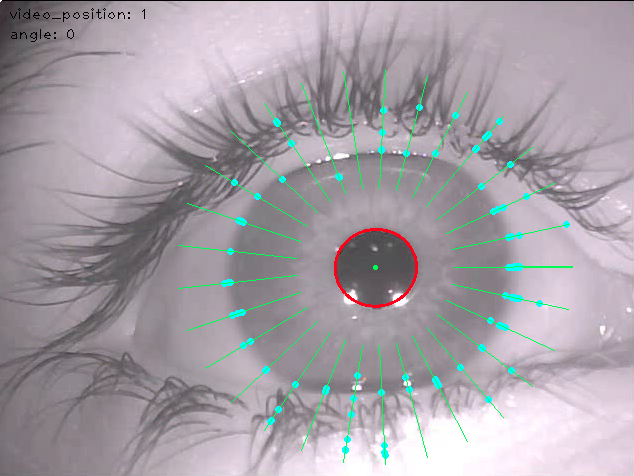
\includegraphics[width=\textwidth]{final/images/iris_samples.png}
		\caption{Samples}
		\label{subfig:iris_samples}
	\end{subfigure}%
	~
	\begin{subfigure}[b]{0.5\textwidth}
		\centering
		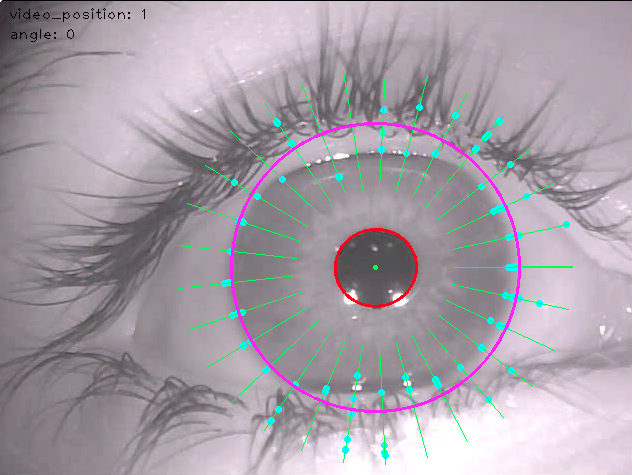
\includegraphics[width=\textwidth]{final/images/iris_estimation.png}
		\caption{Estimation}
		\label{subfig:iris_estimation}
	\end{subfigure}
	
	\caption{Iris Estimation}
\end{figure}

Iris detection works a bit differently than pupil and glint detection in that it works with the assumption that the pupil was detected correctly and therefore there should be an iris to be found. So the detector just counts different votes for individual circle radii and picks the highest one. Of course the worst case for this is when pupil has been mis-detected and there is at least one corresponding orientation and magnitude for one of the 30 sample lines taken, which is highly probable. In this case the iris will be detected on this radius, even though there is only one vote.


\subsubsection{Glint Detection}

Glint detection is in principle very similar to pupil detection, first we compute k-means to a downsized gray scale image. Since the glint can be considered a flash of light in the eye, we assume that this will the brightest point with the first cluster. 
Therefore, we can use k-means to set the values for the thresholding functions, which are called next. After thresholding we find blobs in the image using contours. We then reject all blobs that are bigger than 0.1\% of the total image area. This ensures that we do not count big bright areas of the image as glints, since glints are usually small. As the last filter we reject all glints that have centers outside of the iris circle which we have calculated in the previous phase. This will leave us only with the glints inside the eye and nothing else.

\begin{figure}[h!]
	\centering
	
	\begin{subfigure}[b]{0.5\textwidth}
		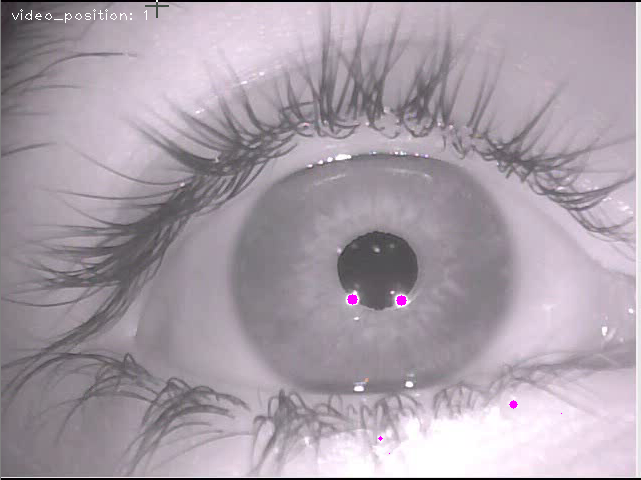
\includegraphics[width=\textwidth]{final/images/glitDetection.png}
		\caption{Glint Detection}
		\label{subfig:glints}
	\end{subfigure}%
	~
	\begin{subfigure}[b]{0.5\textwidth}
		\centering
		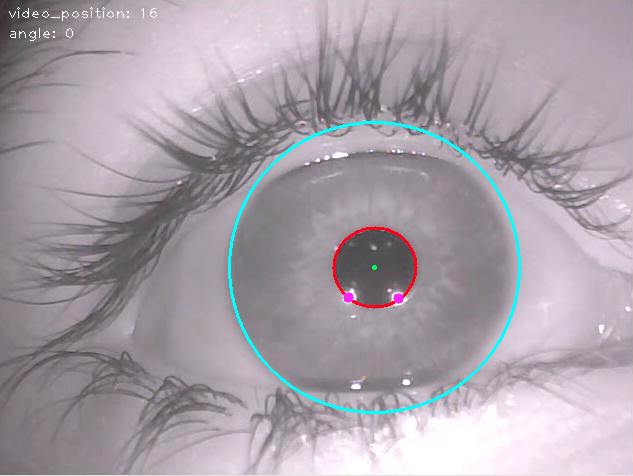
\includegraphics[width=\textwidth]{final/images/final.png}
		\caption{Final Image}
		\label{subfig:final}
	\end{subfigure}
	
	\caption{Glint Detection Phase}
\end{figure}



\subsection{Results}

In order to test our results, we have built a testing framework. The requirements for this were, that it should allow us to quickly and accurately evaluate changes to the detection algorithms. Manual testing is good, but requires us to manually select a sequence and a frame, which can get tedious very quickly.

To combat this, and also get more consistent results, we have defined an array of representative frames from each sequence. We have carefully selected the frames which we had found to cause most problems for our detection algorithms during manual testing. Therefore our representative sample contains the worst-case frames for each sequence (eye looking different directions, challenging light, or eye position). 

On the other hand, we have selected only 5-8 frames per sequence (56 frames together), so the testing can quickly finish and produce representative results. We have also made sure that all of the frames in question do contain the pupil (i.e no frames with closed eye or where no detection can be made) The testing script also writes all the frames with pupil/iris/glint detections drawn on top into a folder for further (manual) inspection.

Unfortunately we cannot automatically test if a detection is correct, because we have no reference implementation, so the correction still has to be evaluated manually. But what we can detect automatically is the number of detected results (i.e what percentage of images that contained eye have had at least something detected by our implementation). This can at least give us  at least preliminary results, if we assume that most of the detected pupils are correct, we should get a good idea about the results from this alone. Of course this does not mean that we can solely rely on this automatic testing and therefore manual verification still has to be performed.

\begin{table}[h!]
	\center
	\begin{tabular}{ |l|l|l|l| }
		\hline
		Sequence & Frames Evaluated & Pupil Detected & Detected Correctly \\ \hline
		
		eye1.avi 	& 5 	& 5 (100\%)	& 5 (100\%) \\
		eye2.avi 	& 6 	& 6 (100\%)	& 6 (100\%) \\
		eye3.avi 	& 8 	& 8 (100\%)	& 5 (62.5\%) \\
		eye4.avi 	& 8 	& 6 (75\%)	& 6 (75\%) \\
		eye5.avi 	& 6 	& 5 (83.3\%)	& 2 (33.3\%) \\
		eye6.avi 	& 7 	& 7 (100\%)	& 5 (71.43\%) \\
		eye7.avi 	& 8 	& 8 (100\%)	& 8 (100\%) \\
		eye8.avi 	& 8 	& 5 (62.5\%)	& 5 (62.5\%) \\
		
		\hline
		Total 	& 56 & 50 (89.29\%) & 42 (75\%) \\ 
		\hline
	\end{tabular}
	\caption{Semi-Automatic Evaluation of the Detection Algorithm}
	\label{tab:eval}
\end{table}

The Table \ref{tab:eval} shows how many frames were evaluated per sequence, how many of those frames have had something detected by our algorithm (counted automatically during testing) and lastly, how many of the frames have the pupil detected correctly \footnote{By definition of our sample, all frames have the pupil present, so it is an error of the algorithm if it is not detected} (this has been done by manual inspection of all generated frames, i.e pupil detected is right size and corresponds to the actual location of the pupil in the image). 

\begin{figure}[t]
	\centering
	
	\begin{subfigure}[b]{0.5\textwidth}
		\centering
		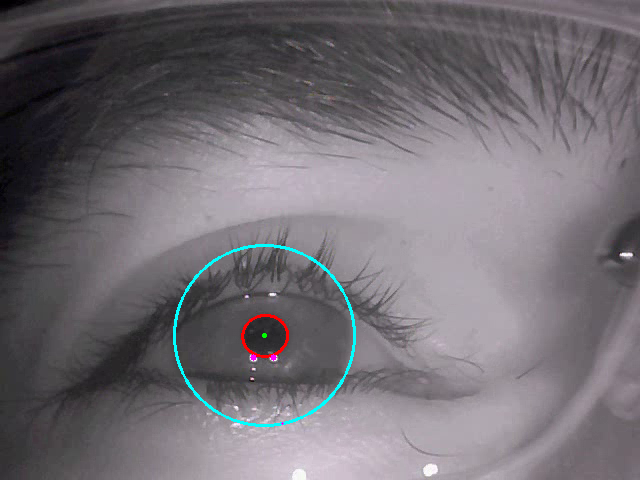
\includegraphics[width=\textwidth]{final/images/good1.png}
		\caption{Eye Squinting}
		\label{subfig:squinting}
	\end{subfigure}%
	~
	\begin{subfigure}[b]{0.5\textwidth}
		\centering
		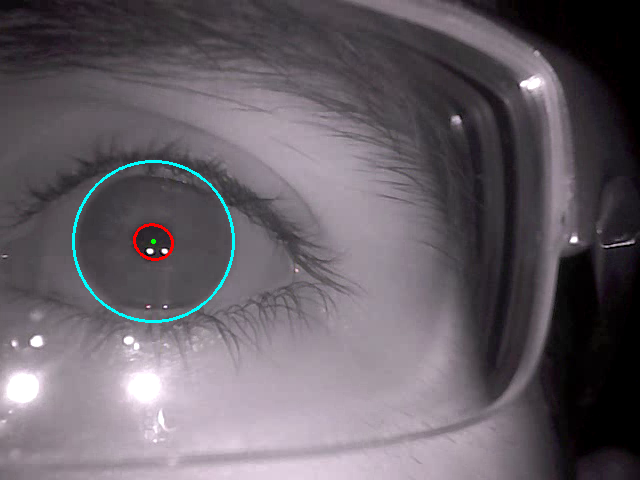
\includegraphics[width=\textwidth]{final/images/good2.png}
		\caption{Challenging Light}
		\label{subfig:challenging_light}
	\end{subfigure}
	
	\begin{subfigure}[b]{0.5\textwidth}
		\centering
		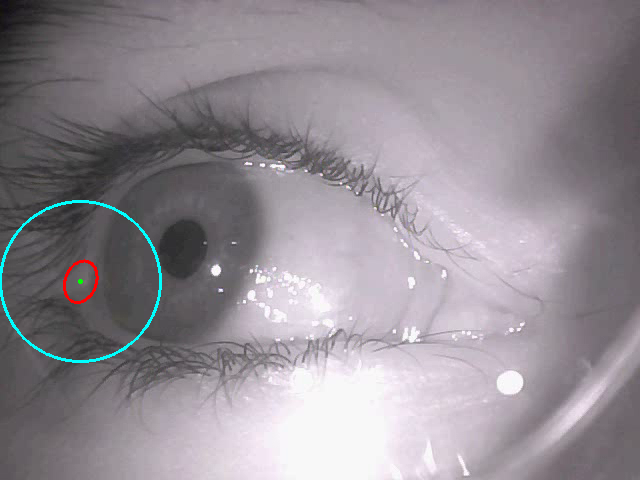
\includegraphics[width=\textwidth]{final/images/wrong1.png}
		\caption{Wrong Detection}
		\label{subfig:wrong1}
	\end{subfigure}%
	~
	\begin{subfigure}[b]{0.5\textwidth}
		\centering
		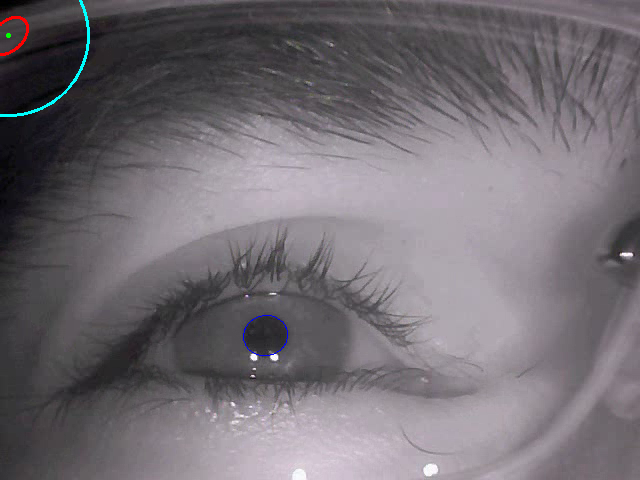
\includegraphics[width=\textwidth]{final/images/wrong2.png}
		\caption{Ordering By Extend}
		\label{subfig:extend}
	\end{subfigure}
	
	\caption{Results}
	\label{fig:results}
\end{figure}

Figure \ref{fig:results} shows good results in the first row (images (a) and (b)) under challenging conditions, as well as wrong results that can occur in row two (images (c) and (d)). In Figure \ref{subfig:extend} you can see a blue circle around the pupil, which is an alternative blob that has been considered by the algorithm, but was most likely rejected because the closing in combination with glints have increased its extend in comparison with the other candidate.

\subsubsection{Discussion}
In the following text we look at the weaknesses of our algorithm, why it does not work in all frames, and how it could be improved. We look at three interesting points of view from which the work could be improved. First we look at performance, where we evaluate what could be done better to improve performance, second and third we discuss false positives and negatives, which occurred during our testing, what reasons there were for this and how could the algorithm be improved.

Regarding performance in time, our algorithm is not achieving very good results, primarily because we focused on the detection and code readability, and due to shortage of time we could not work on the speed optimizations as we would have liked. However we can mention some of the sacrifices we have made to improve code readability and ease of handling during testing. 
For example in various parts of the algorithm we use the gray scale image, which we most of the time just calculate again, instead we could either implement some sort of cache or pass the gray scale image around and only generate it once. Similar story is with k-means image. We use the same algorithm in pupil and glint detection, yet these two do not share the results, which they should.

False positives are cases where a pupil is detected in a place where it is not actually supposed to be. We have found that this usually occurs when there are very dark areas in the image. This confuses the k-means, producing the darkest region that does not necessarily contain the pupil, at which point the whole algorithm is destined to fail. It will pick a blob that best resembles the pupil out of those available and try to work with that, producing wrong results. 
A solution we have tried to combat this problem is overlaying a transparent-to-white radial gradient from the center of the image to suppress the dark areas around image edges. But what we found was that even though the number of detections in sequences that were most affected by the above described problem went up, the overall results over all of the sequences were worse. So we decided against that improvement. However it still might be warranted to selectively apply it to only some of the sequences, if it can be safely assumed that the pupil stays near the center of the frame and there are dark areas near the edges of the frame.

False negatives are produced when a pupil should have been detected, but was not. These cases can be caught by our automated testing, because all of the frames being tested should contain a pupil. This is of course very similar to the previous case with k-means, but we have to manage limiting this problem using the iterative lowering of k-means parameter.

One idea, if the detection was speedier, would be to actually compare the detected positions with the previous frame, this could improve the results when the pupil is suddenly detected in the wrong part of the image, but might have a negative impact, when the first detection is wrong, then all the subsequent detections could be wrong as well.


\subsection{Conclusion}
In the beginning we have set out to build an eye tracker. We have constructed an eye tracker by iteratively building up detectors for pupil, iris and glints. We have described this process in the Method section. Next, we have built a test suite to evaluate the results we got from our eye tracker. We have talked about this in the Results chapter, where we also discussed the performance of the algorithm both in terms of speed and accuracy.

The overall result that we have managed to achieve with our algorithm is 42 (75\%) of correctly identified pupils/iris on our challenging sample of 56 tested images.

In conclusion, we can therefore state that our eye tracker is performing reasonably well in terms of accuracy, but is experimenting some lacks in terms of speed of execution, where it still has some problems. Most of these problems can most likely be solved by re-architecting the code to reuse already performed computations and remember results between frames.

\section{Homography}
\subsection{Person Map Location}

In this section, the task was to use linear algebra to map a person walk from video source taken at an angle to the overview map of the ITU. We have been given a video file where a person can be seen walking in the atrium of the IT University of Copenhagen, trace data that represents the person's position in each frame in the video, and an overview map of the ITU. We have also had a tool at our disposal that allowed us to obtain the homography matrix from the video to the map. 

We started by obtaining the homography matrix. We have specified four points in a frame of the provided video, and then we have tried to select the exact same points on the overview map. All of the four points had to lay on a plane, because a homography matrix describes the relation between two views of the same plane. We also need at least four points, because otherwise (e.g with three points) we would only be able to describe an affine transformation, not a projection. It is important to note, that since the entire video sequence of the walk is taken from a stationary camera (i.e the camera does not move during the exposition), and because the overview map of ITU is also not changing, it is sufficient to calculate the homogaphy once for the entire sequence. Otherwise we would need to recalculate it for each frame when the relative position of the camera and the ground plane has changed.

\begin{figure}[h!]
	\centering
	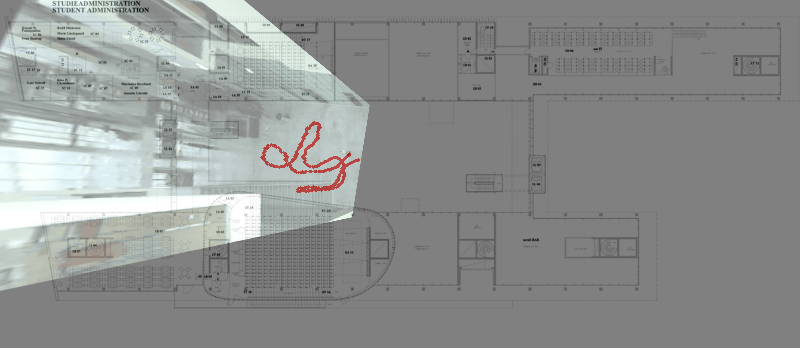
\includegraphics[width=\textwidth]{final/images/trace_map.png}
	\caption{Trace Map}
	\label{fig:trace}
\end{figure}

Using the obtained homography matrix we have been then able to project the video image onto the overview map of ITU which can be seen in the Figure \ref{fig:trace}. Using the trace data provided we have then been able to position the person in the overview map. We have taken the center point of the bottom edge of the rectangle describing the person's legs. This point should always be on the ground and therefore should guarantee the best approximation of the person's actual position (as opposed to the head for example, which would form a triangle between head, legs and a point defined by camera angle further away from the camera on the floor, yielding an inaccuracy of around the person's height at this camera angle).

\begin{equation}
	L = H \cdot P
	\label{form:homography}
\end{equation}

Figure \ref{fig:trace} has been produced by drawing a red point for each frame using the Formula \ref{form:homography} where L is the person's location in the overview map, H is the pre-calculated homography matrix, and P is a point corresponding to the middle of the bottom edge of the rectangle describing the person's legs.

\begin{figure}[h!]
	\centering
	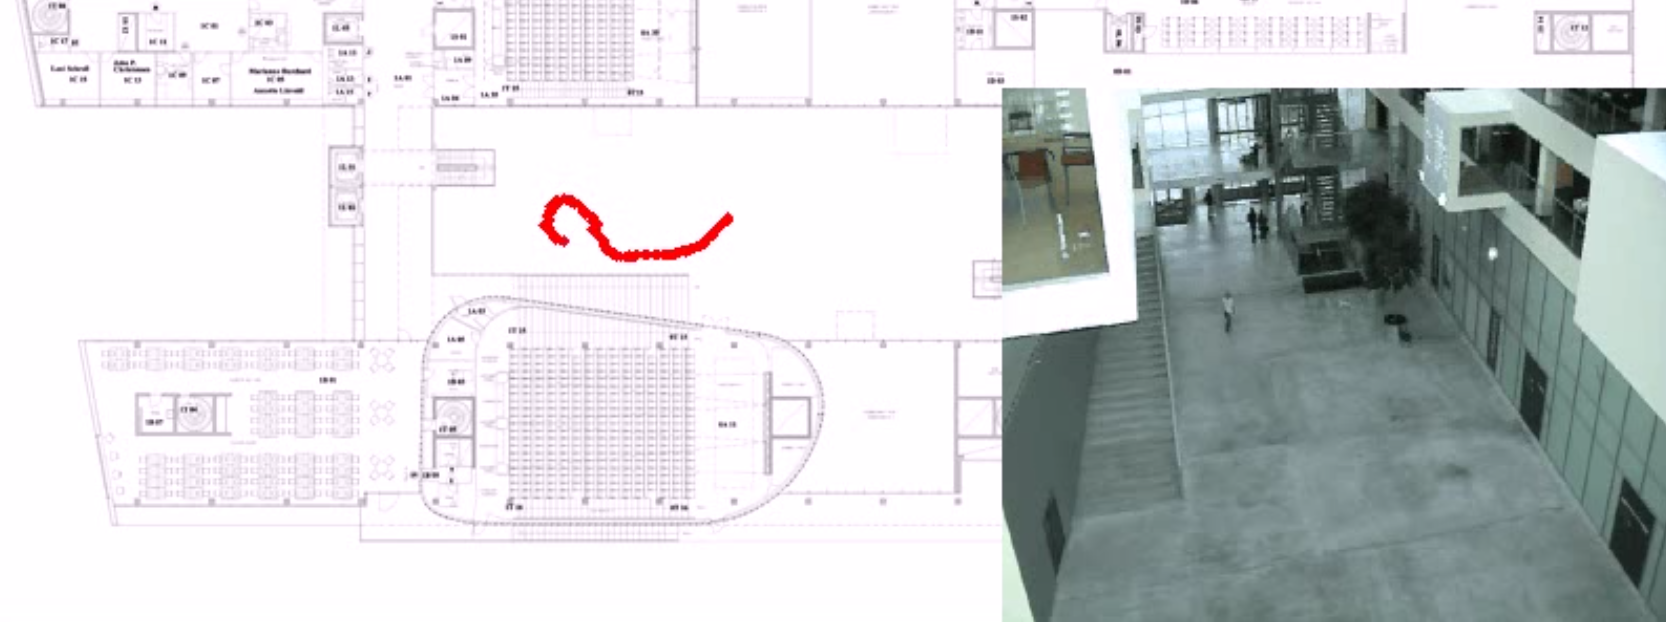
\includegraphics[width=\textwidth]{final/images/personlocationvideo.png}
	\caption{Video Trace}
	\label{fig:video_trace}
\end{figure}

The reason this mapping is useful, is that in the overview map it is easier to see the person's position on the ground plane. On the other hand, depending on the camera angle relative to the ground plane, the accuracy of the estimation can vary depending on the distance from the camera.

\subsection{Linear Texture Mapping}

This section is divided into three parts, first we will look at how to overview the ITU logo on the image sequence of universities ground floor. Then we look at how we can overview a texture on a moving object. In the third part we tried to be sure that the texture looks realistic compared to the geometry of the texture.

\subsubsection{Ground Floor}

In this part we tried to overview the ITU logo on the image sequence of ground floor. For this we used the same code from simpleTextureMap function and declare the texturemapGroundFloor method with the implementation for overviewing the logo on each frame of the sequence by using four mouse input points from the first frame.

\begin{figure}[h!]
	\centering
	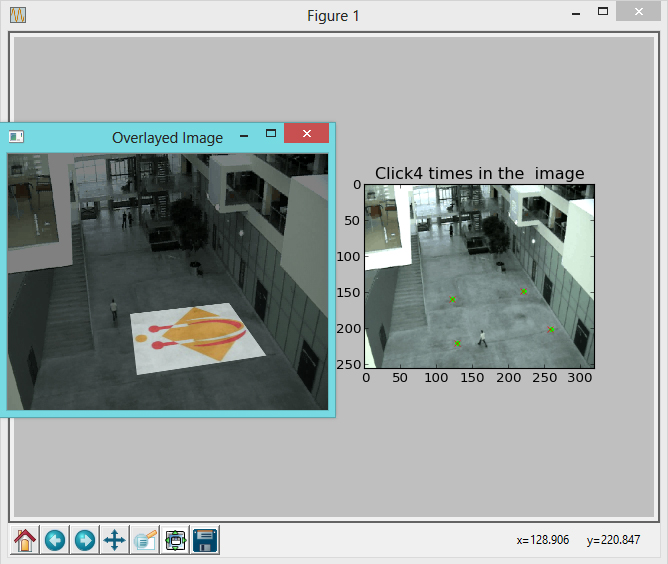
\includegraphics[width=\textwidth]{final/images/linearmapping.jpg}
	\caption{Linear Mapping}
	\label{fig:linearmapping}
\end{figure}

\subsubsection{Moving object}

In the second part of linear texture mapping we tried to experiment with texture mapping on image sequences where the objects move. We have been given some video files where a grid pattern moves in it. The aim is to mapping a texture on the pattern that will move with it. For the start we found the pattern corners with findChessboardCorners function and used it for calculating the homography matrix and overview the logo on the pattern. So for each frame we get a new homography matrix and new texture mapping. Our implementation weakness is that in some frames that it can't detect corners of the pattern it will fail because we used corners location to mapping the logo.

\begin{figure}[h!]
	\centering
	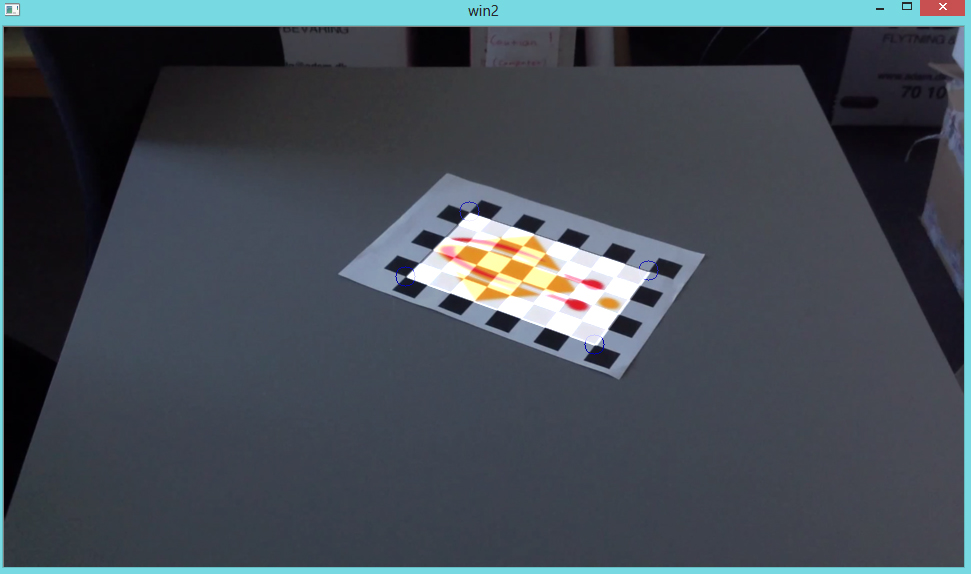
\includegraphics[width=\textwidth]{final/images/linearmapping2.jpg}
	\caption{Moving Pattern}
	\label{fig:movingpattern}
\end{figure}

\subsubsection{Ensuring a correctly placed texturemap}

The last part, depicted in Figure \ref{fig:realistictexturing}, is realistic texture placement on the ground floor. We start by selecting a point in the overview map. Next, we calculate placement of corner points in the overview map. We regard the selected point as a center, and then we calculate the corners from provided scale factor and texture dimensions.

We are then able to obtain the positions of the corners in the video image by calculating the dot product of the inverse of the homography $H_{G}^{M}$ and the positions of the points in the overview map. We can then calculate the homography between the texture T and ground plane in the video image G $H_{T}^{G}$. This allows us to position the texture consistently with the ground plane just by selecting a single point.

\begin{figure}[h!]
	\centering
	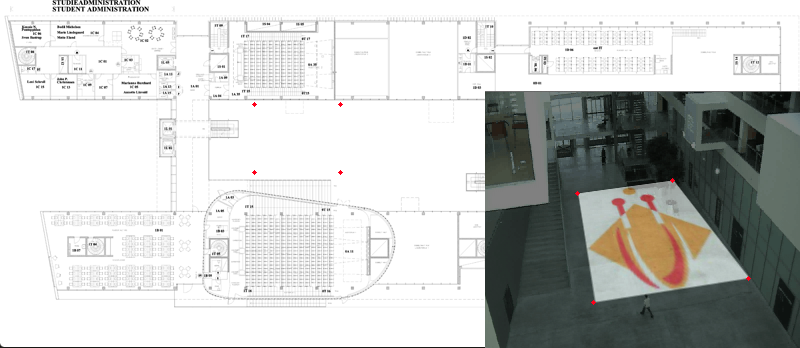
\includegraphics[width=\textwidth]{final/images/realistictexturing.png}
	\caption{Realistic Texturing}
	\label{fig:realistictexturing}
\end{figure}

\subsection{Camera Calibration and Augmentation}

This section is divided into two parts, first we will look at how we obtained proper camera calibration and distortion coefficients. Then we look at how we used this information to augment the image obtained from the camera with a projected cube.

\subsubsection{Camera Calibration}

During the camera calibration phase we aim to obtain intrinsic camera parameters. This is divided into two parts, first there is a camera matrix K (see Equation \ref{eq:cameramatrix}) which describes the intrinsic properties of the camera, and then there are distortion coefficients which we do not represent in the linear camera model, but they affect the image nonetheless. 

The R|t part is the rotation/translation matrix. This are the extrinsic properties of the camera like its rotation and translation in the world.

P is a point in the 3D space that we want to project onto the 2D image obtained by the camera. 

C represents the 2D coordinates in the image produced by the camera when P is projected.

\begin{equation}
	\underbrace{
		\begin{bmatrix}
			u \\
			v \\
			1
		\end{bmatrix}
	}_\text{C}
	=
	\underbrace{
		\begin{bmatrix}
			f_{x} & 0 & t_{x} \\
			0 & f_{y} & t_{y} \\
			0 & 0 & 1
		\end{bmatrix}
	}_\text{K}
	\cdot
	\underbrace{
		\begin{bmatrix}
			R_{1,1} & R_{1,2} & R_{1,3} & t_{x} \\
			R_{2,1} & R_{2,2} & R_{2,3} & t_{y} \\
			R_{2,1} & R_{2,2} & R_{3,3} & t_{z}
		\end{bmatrix}
	}_\text{R|t}
	\cdot
	\underbrace{
		\begin{bmatrix}
			X \\
			Y \\
			Z \\
			1
		\end{bmatrix}
	}_\text{P}
	\label{eq:cameramatrix}
\end{equation}

The calibration is obtained in OpenCV by repeated exposures containing the calibration pattern. Based on this, OpenCV calculates the intrinsic camera properties and returns them as K and distortion coefficients. It should be noted that unless the camera allows for focal length manipulation, the intrinsics will not change. So it makes sense to just calibrate once and save the calibration into a file which then can be reused.

\subsubsection{Augmentation}

In the next part we have used the calibration obtained in the previous section to augment the image with a 3D object (cube) Figure \ref{fig:augment}. The basis for this was to obtain a homography from one virtual camera to another. 

\begin{figure}[h!]
	\centering
	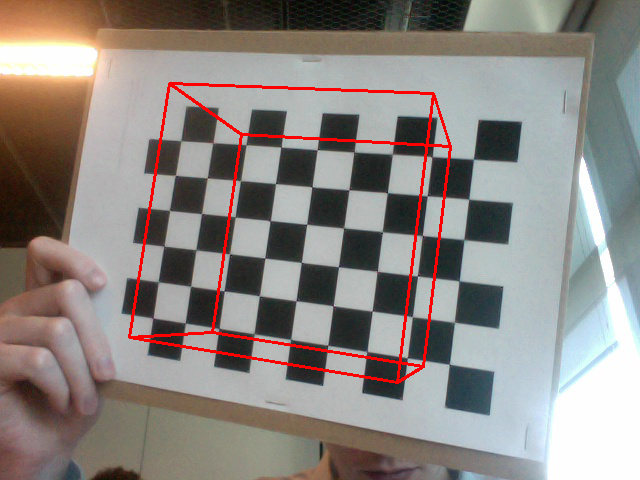
\includegraphics[width=\textwidth]{final/images/augmentation1.png}
	\caption{Augmented image}
	\label{fig:augment}
\end{figure}

First we have constructed a camera that would look at just the chessboard pattern. Then we have calculated the positions of some select corners in that pattern, and using the same corners in the same pattern in the image obtained from the video, we have been able to estimate a homography that would describe the relationship between the two.

From that we have been able to re-construct the camera that was essentially used to take the video image. we have had the calibration from before, and now using the homography we have been able to calculate the rotation and translation matrices from the Equation \ref{eq:solvingforrotation} where we obtain $r_{1}$, $r_{2}$ and t as dot product of the inverse of K, the calibration matrix, and H, the homography between the two planes. $r_{3}$ can be calculated as a cross product of $r_{1}$ and $r_{2}$.

\begin{equation}
	K^{-1}H = [r_{1}, r_{2}, t]
	\label{eq:solvingforrotation}
\end{equation}

Now using the projection matrix of the second camera, we can project points in the 3D space onto the final image, so that they appear as if they were in the scene. And since the homogrpahy is calculated from one chessboard to another, the points are anchored the position of the chessboard.


\pagebreak
\section{Augmented Reality}

\subsection{Introduction}

This assignment has been divided to two main parts: drawing a cube and shading it. In the first part the emphasis was more on the mathematics behind the camera calibration, homographies and projections, whereas in the second part we have focused on calculating shading of the textured cube. Similarly to the previous assignments, we used Python and OpenCV as a toolkit.

In the following text we describe the steps we took to complete the assignments. Each step is building on top of the previous in a natural progression. We begin by describing how we used camera calibration to establish world coordinates, next we describe the steps necessary to project a wireframe cube into this world, followed by projecting a textured version of the cube, and backface culling to remove the faces not visible from the camera perspective.

In the second part of the assignment we enhance the textured cube from the first part by applying the Phong shading algorithm for a single light source


\subsection{Camera Calibration}
We started out by calibrating the camera using a chessboard pattern provided by the OpenCV library. This allowed us to compute both, intrinsic and extrinsic camera parameters as well as distortion coefficients for the camera. 

\begin{equation}
	P = K \begin{bmatrix} R|t \end{bmatrix}
\end{equation}

The intrinsic camera parameters \textit{K} do not change in time, because the camera we used does not have the ability to change the focal length of the lens, so it makes sense to store this data for later. 

The extrinsic parameters (\textit{R} and \textit{t}) on the other hand change with the position of the chessboard pattern.

Intrinsic and extrinsic parameters together make camera projection matrix \textit{P}. We use this matrix later to calculate homography between the first view we used to store the camera calibration and subsequent views in the rendering.

To verify that \textit{P} is correct we projected chess points on the first camera view. As you can see in the Figure \ref{subfig:chesspattern} all the points have been projected exactly into the right position.
 
 \begin{figure}[h!]
	\begin{subfigure}[b]{0.5\textwidth}
		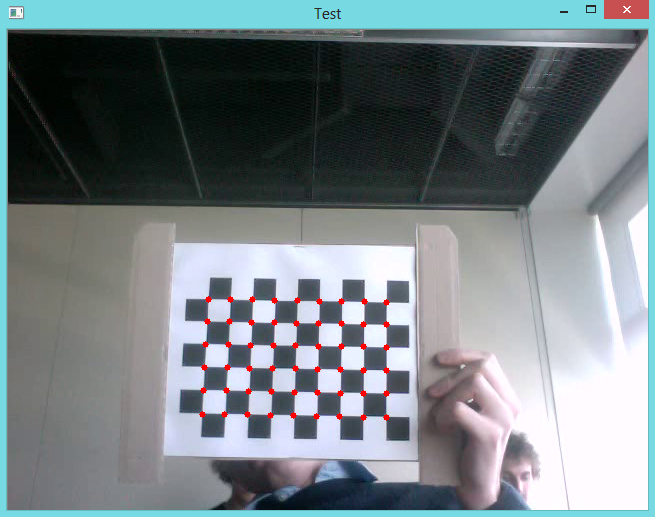
\includegraphics[width=\textwidth]{final/images/patterndot.jpg}
		\caption{Chessboard}
		\label{subfig:chesspattern}
	\end{subfigure}
	~
	\begin{subfigure}[b]{0.5\textwidth}
		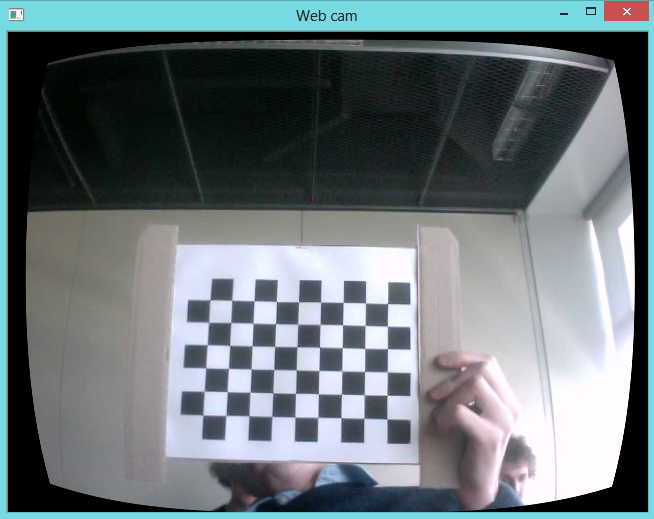
\includegraphics[width=\textwidth]{final/images/undistort.jpg}
		\caption{Undistort}
		\label{subfig:undistort}
	\end{subfigure}
	
	\caption{Camera Calibration}
\end{figure}
 
In the last step of this part we tried to undistorted the image by using the (cv2.undistort) function. (see Figure \ref{subfig:undistort}). Using the chessboard, OpenCV has been able to calculate camera distortion coefficients, which we have stored for later use as well.

\subsection{Augmented Cube}
In this section, we calculated the full camera matrix in each frame and we used that for projecting a 3D cube into that frame. After that we tried to do the texture mapping on the faces of the cube we projected.

We tried two methods for calculating the projection camera. First method uses chessboard obtained from an arbitrary "first" image, and computes the homography between the first frame and the currently processed frame. It then uses the homography to construct the projection matrix for the camera. The second method uses just the chessboard pattern in the current frame to establish the world origin and relate the camera position towards it.

The second method gives us a better result, because the first method computes the homography between two frames and because the frames can have relative distortion with each other and an absolute distortion it will slightly worse result.

Now that we found the camera matrix with both methods for testing them we tried to project the chesspattern points in the world coordinate system to the current camera view. All points were projected to the right place in the image so we moved to the next step.

In this step we drew the world coordinate axes attached to the chesspattern plane and then we projected the cube into the current view again attached to the pattern plane. In order to do this, we had a representation of the cube in object coordinates, and we have positioned it in the world without any translation, rotation or scaling. Thanks to this, it was possible for us to treat the coordinates of the cube object coordinate system as if they were in the world coordinate system. Otherwise we would have to transform them from object coordinate system into world coordinate system.

 \begin{figure}[h!]
	\centering
	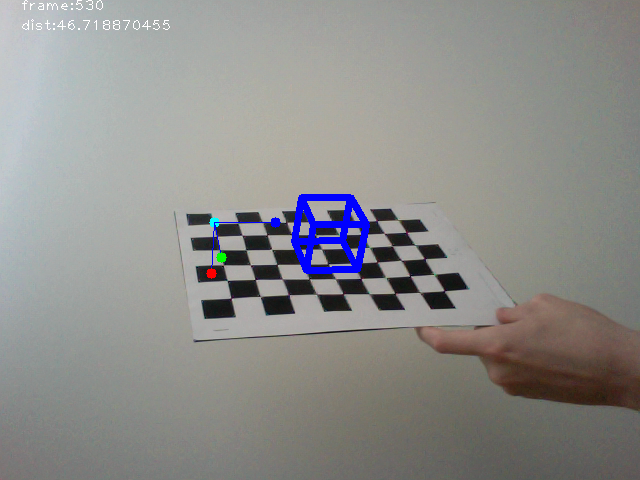
\includegraphics[width=\textwidth]{final/images/wireframe.png}
	\caption{Wireframe Cube}
	\label{fig:wireframe}
\end{figure}

To draw a wireframe model in Figure \ref{fig:wireframe} we simply take a pair of points from the cube that form an edge, project them using the projection matrix we calculated before to obtain their positions in the 2D image and then just draw a line between them.

\subsection{Back-face Culling and Texture Mapping}

To texture our wireframe model, we first calculate the homography between the texture (2D image) and a face of the cube as it is projected in the 2D final image. We then use this homography to perspective warp the texture into the final image. See Figure \ref{subfig:texture}. But this is obviously not right, some faces overlap others randomly. We solve this by a technique called back-face culling.

Back-face culling is a technique we have employed to address the problem that appears when we render the whole cube. In the 2D view you cannot see all 5 textured faces of the cube at once. It is only possible to see one to three faces at any given time. Therefore some faces we render are redundant. All faces are drawn in the order in which the list containing their names is processed, so it is the same order always. Therefore the faces that are drawn later occlude faces drawn earlier, even though logically they should be behind them. 

To address this problem, a simple technique has been developed, where we determine the angle between the camera and a face, and based on that we decide whether or not to show the face. First we compute the unitary normal vector of the face. We take three points from the face, since we assume that the face is composed of four coplanar points, it does not matter which three we take, but the order does matter, because with wrong order we will get a normal that faces the other way (inside the cube). We then construct displacement vectors between two point pairs of the three points, and calculate the cross product of these vectors. As the last step we transform the obtained vector to get a unitary vector. 

Similarly we compute a vector from camera center and the center of the face we are comparing. We transform this vector to unitary as well. We can calculate the angle between the two vectors. If this angle is greater than 90 degrees, we know that the face is facing away from the camera, and we therefore do not draw it.

 \begin{figure}[h!]
	\begin{subfigure}[b]{0.5\textwidth}
		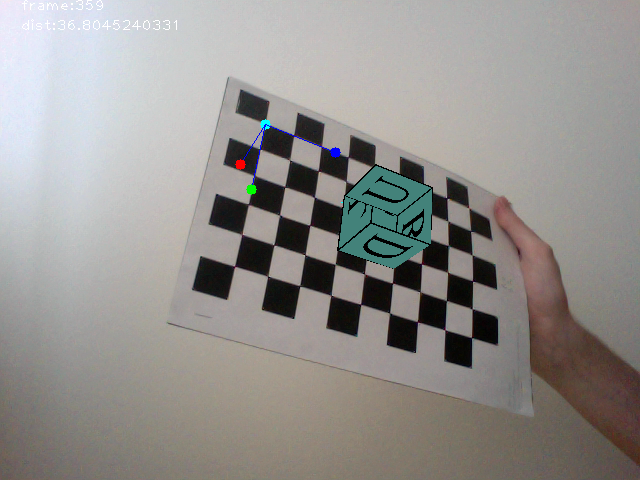
\includegraphics[width=\textwidth]{final/images/culling.png}
		\caption{Texture Mapping}
		\label{subfig:texture}
	\end{subfigure}
	~
	\begin{subfigure}[b]{0.5\textwidth}
		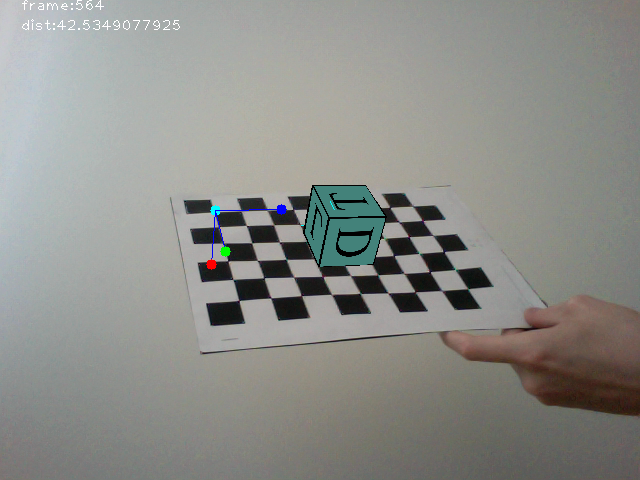
\includegraphics[width=\textwidth]{final/images/texture2.png}
		\caption{Back-face Culling}
		\label{subfig:backculling}
	\end{subfigure}
	
	\label{fig:texturing}
	\caption{Backface Culling and Texture Mapping}
\end{figure}

\subsection{Shading}

Shading is a process that is often applied to 3D rendered objects to make them appear more realistic by modeling  how light interacts with them. In the code we have implemented, we have used the Equation \ref{eq:shading}. In the equation \textit{I} is final illuminated texture of a face, \textit{T(u, v)} is the texture of the face with dimensions s and t. \textit{L\textsubscript{a}} is the ambient illumination, \textit{k\textsubscript{a}} is the ambient component of the object's material. \textit{L\textsubscript{l}} is light intensity, \textit{k\textsubscript{d}} is the diffuse component of the material. \textit{n} is the face normal vector. \textit{k\textsubscript{s}} is the specular component of the material. \textit{v} is the viewer vector and \textit{r\textsubscript{i}} is the reflected light vector. All vectors are unitary.

\begin{equation}
	I=T(u,v)[
	\underbrace{
	L_{a}k_{a}
	}_\text{Ambient}
	+
	\underbrace{
	k_{d}\sum\limits_{i}L_{i}max(n\cdot l_{i},0)
	}_\text{Diffuse}
	+
	\underbrace{
	k_{s}\sum\limits_{i}L_{i}(r_{i}\cdot v)^\alpha
	  }_\text{Specular}
	]
	\label{eq:shading}
\end{equation}

This equation differs slightly from what has been implemented in our report, because it allows for multiple light sources, whereas we have only implemented one light source. On the other hand both the equation and our implementation assume the material is uniform, while it could easily be a texture.

To shade the individual faces in our project, we used a low resolution (10$\times$10) texture that we have multiplied with the texture calculated from before. We have implemented two different approaches to shading, the flat shading model and Phong shading model. In both models, the underlying equation is the same (Figure \ref{eq:shading}), but there are differences in how it is applied.

In the flat shading model, we only need to calculate one diffuse and specular value per face, and apply it to the whole face.

In contrast, Phong shading model assigns each pixel in our light texture a different normal, calculated using bilinear interpolation from corner normals of the currently evaluated face. The corner normals are calculated by averaging the normals of all neighboring faces. The result of all of this is that there is a smooth transition between normals calculated for points along the face. This allows us to draw objects with relatively small face counts (and therefore smaller and easier to store and manipulate) easily and with nice smooth surface. 

This means that we can then use this normal to calculate the illumination at a single point of the face texture to obtain a smooth gradient corresponding to diffuse and specular light. 

All that remains is then to combine the illumination texture with the original texture to shade the face and project it to create the final image. Of course this is repeated for every face.

We have also implemented different light positions. It is possible to click into the camera window and select a new position for the light, which is by default positioned in the camera center, see Figure \ref{subfig:extra1} and \ref{subfig:extra2}. 

 \begin{figure}[h!]
	\begin{subfigure}[b]{0.5\textwidth}
		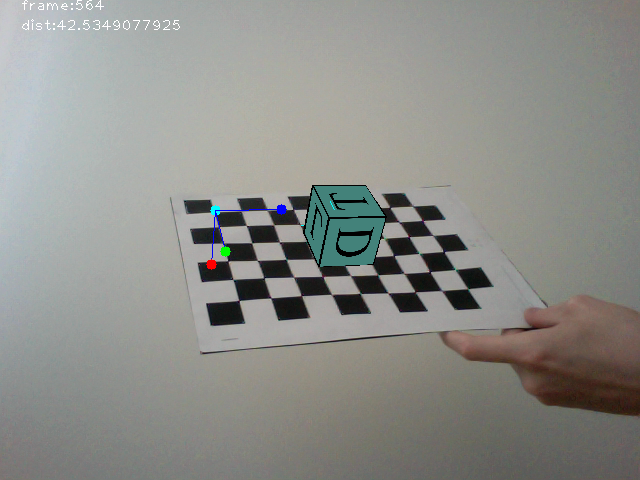
\includegraphics[width=\textwidth]{final/images/texture2.png}
		\caption{Plain Texture Mapping}
		\label{subfig:plaintexture}
	\end{subfigure}
	~
	\begin{subfigure}[b]{0.5\textwidth}
		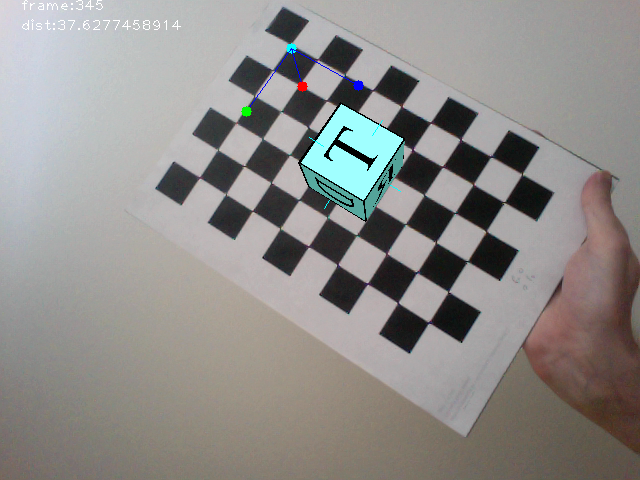
\includegraphics[width=\textwidth]{final/images/flat.png}
		\caption{Flat Shading}
		\label{subfig:flatshading}
	\end{subfigure}
	~
	\begin{subfigure}[b]{0.5\textwidth}
		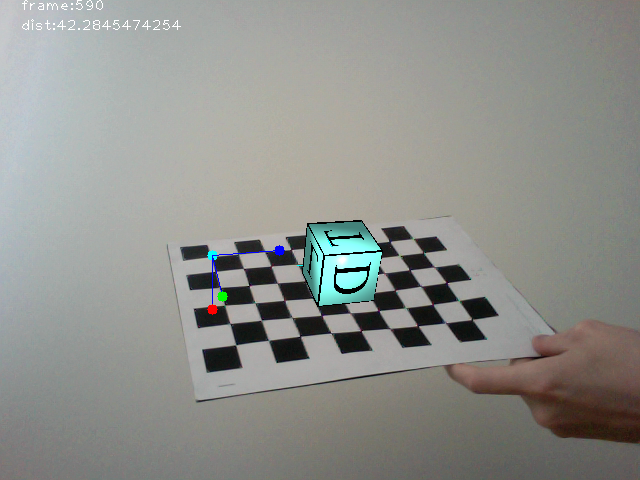
\includegraphics[width=\textwidth]{final/images/phong1.png}
		\caption{Phong Shading}
		\label{subfig:phongshading}
	\end{subfigure}
	~
	\begin{subfigure}[b]{0.5\textwidth}
		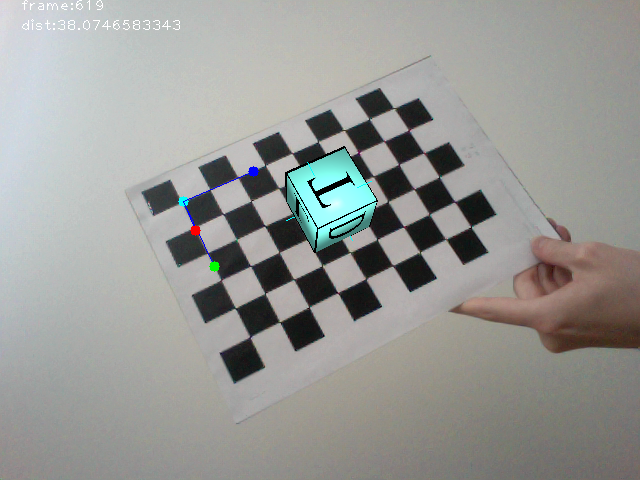
\includegraphics[width=\textwidth]{final/images/phong2.png}
		\caption{Phong Shading 2}
		\label{subfig:phongshading2}
	\end{subfigure}
\end{figure}
 \begin{figure}[h!]
	\begin{subfigure}[b]{0.5\textwidth}
		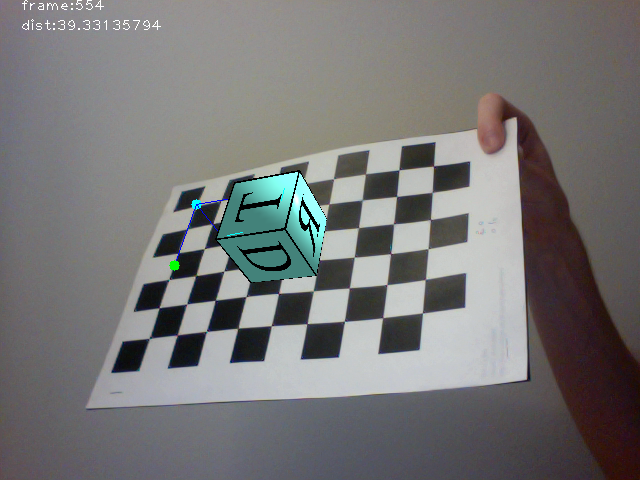
\includegraphics[width=\textwidth]{final/images/extra1.png}
		\caption{Light Position Top Right}
		\label{subfig:extra1}
	\end{subfigure}
	~
	\begin{subfigure}[b]{0.5\textwidth}
		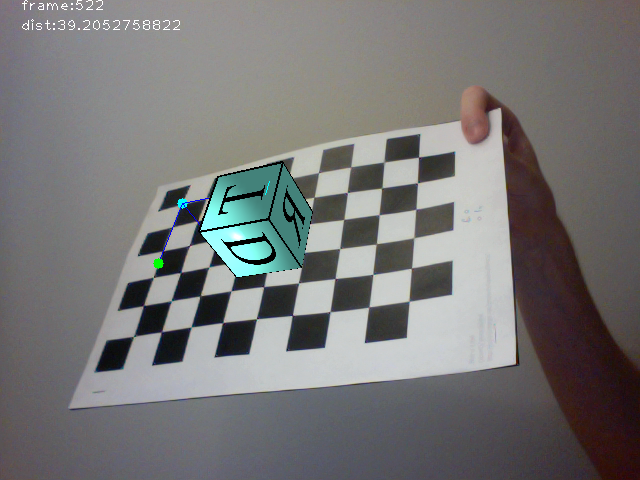
\includegraphics[width=\textwidth]{final/images/extra2.png}
		\caption{Light Position Bottom Left}
		\label{subfig:extra2}
	\end{subfigure}
	
	\label{fig:texturing}
	\caption{Shading}
\end{figure}

\subsection{Conclusion}

In this assignment we have worked with various techniques that are in use in the field of computer graphics. We have looked at how homographies are useful in calculating camera projection matrices and how those matrices are useful in projecting 3D world onto a 2D image. We have tried out texturing a 3D object and we have explored the intricate mathematics of shading models. We found it very useful and applicable in many areas, such as augmented reality, 3D programming, etc. In the end we have been successful in implementing all the methods and techniques described, and we have deepened our knowledge of the 3D concepts in use.



\section{Conclusion}


\bibliography{refs}
\bibliographystyle{plain}

\nocite{*}

%%% End document
\end{document}